%AL BEGIN unnecessary stuff
\color{cyan}
\subsection*{All the stuff below this line not needed !!!}
Error definitions:\\
$\lambda$ = latitude, $t$=time, \\
$N_t$ = number of bins (time), \\
$N_\lambda$ = number of bins (latitude), \\
$N_P$ = number of \fff measurements in a patch, \\
$\overline{X}$ indicates average over time, \\
$f(\lambda,t)$ = \fff strength (unbinned)\\
$f_P(\lambda,t)$ = \fff strength in latitude / time bins (patches)\\
$\overline{f}(\lambda) = 1/N_t \sum_t f(\lambda,t)$ = temporal mean of the \fff strength (unbinned)\\ 
$f'=f-\overline{f}$ is the fluctuation around the temporal mean, i.e. the solar cycle dependence of the \fff (unbinned)\\
$\overline{f_P}(\lambda) = 1/N_t \sum_t f_P(\lambda,t)$ = temporal mean of 
\fff strength (in lat / time bins), \\
$f'_P=f_P-\overline{f_P}$ is, correspondingly, the binned fluctuation\\

%AL added this
The following 4 definitions represent what is plotted in \fig{butterfly_lat_old}:
\begin{itemize}
\item sdev(cycle) 
%AL added the subsript cyc to indicate that this sigma is computed  over the whole cycle, and to distinguish it from \sigma_P
%$\sigma(\lambda)$ 
$\sigma_{\mbox{cyc}}(\lambda)$ 
(red shaded area): this quantity displays the variation of the \fff over the solar cycle.
%AL added
the subscript 'cyc' should indicate that this variation includes also the solar cycle variation. This distinguishes it from $\sigma_P$ defined below, which does not contain the solar cycle variation.
\begin{equation}
%MJK I think subscript P is missing from here, and the need for 'cyc' I cannot understand.
%AL correct. The P was missing. I tried to explain the 'cyc'
%\sigma^2_{\mbox{cyc}}(\lambda) 
%AL commented out this:
%\sigma_P^2(\lambda)  = 
%AL and changed it to:
\sigma^2_{\mbox{cyc}}(\lambda) =
\frac{1}{N_t} \sum_{t} \left( f_P(\lambda,t) -\overline{f_P}(\lambda)\right)^2,
\end{equation}
%MJK added this
hence equalling to the rms value of $f'_P$ (without taking the square root). 
%MJK

\item min/max $\sigma_{\mbox{mm}}$: (blue shaded area): this shows the minimum and the maximum  of $f(\lambda,t) - \overline{f}(\lambda)$:
\begin{equation}
\sigma_{\mbox{mm}}(\lambda) = [ \min_t (f(\lambda,t)),  \max_t (f(\lambda,t)) ] -\overline{f}(\lambda)
\end{equation}

\item min/max (mean) $\overline{\sigma}_{\mbox{mm}}$: (green shaded area): this shows the mean minimum and maximum  of $f(\lambda,t) - \overline{f}(\lambda)$:
\begin{equation}
\overline{\sigma}_{\mbox{mm}}(\lambda) = [ \overline{ \min_t (f(\lambda,t)) }, \overline{ \max_t (f(\lambda,t)) }] -\overline{f}(\lambda)
\end{equation}

\item mean(sdev(patch)) $\overline{\sigma_P}$ (error bars): the standard deviation of the \fff strength
%AL added this
($f(\lambda,t)$)
%AL
 is computed individually for all lat / time bins. This quantity  ($=\sigma_P(\lambda,t)$) is then averaged over time:
\begin{eqnarray}
\overline{\sigma_P}(\lambda) &=&  \frac{1}{N_t} \sum_{t}  \sigma_P(\lambda,t) \mbox{, with} \\
\sigma_P^2(\lambda,t) &=& \frac{1}{N_P}\sum_{\mbox{patch}} ( f(\lambda,t)
- f_P(\lambda,t) )^2,
\end{eqnarray} 
%AL added this
where $\sum_{\mbox{patch}}$ indicates the summation over all \fff strengths within a patch, and $f_P(\lambda,t)$ being the mean \fff strength in this patch. The patch size must be chosen small enough to not contain a significant variation in latitude or solar cycle. 
This quantity $\overline{\sigma_P}(\lambda)$ is displayed as the orange shaded area in \fig{butterfly_lat}.\\
%MJK Added this
This quantity is, therefore, a mean of the $f'_{P, {\rm rms}}$ (so this time also taking the square root) values in individual bins. The problem is that the quantity we are interested in inspecting, and defining the significance of, is now defining the error bar of the measurement. 
%MJK
%AL comment:
%My definition is maybe poor. Yes, I think it should be simply called the 'average rms fluctuation of the \fff strength over 2 months' (in the above plot the patch size in time is 2 months).
\end{itemize}
\subsection*{All the stuff above this line not needed !!!}
\color{black}
%AL END unnecessary stuff

%MJK Cutting this out following the decision from yesterday
%
%AL create this plot with:
ot with:
% %run plot_fmode_butterfly.py -i ../qs_cubes --reread=False --fov 'FFOV_KX0' --show_cos=False --show_cycle=False
\colfigtwocol{butterfly_lat_FFOV_KX0}{Same as \fig{butterfly_lat}, but computed from a wedge of $\pm10^\circ$ around the $k_y$ axis.
%MJK I would not know what is a poloidal component of the f-mode.
%, representing the poloidal component.
\label{butkx0}}

\colfigtwocol{butterfly_lat_FFOV_KY0}{Same as \fig{butterfly_lat}, but computed from a wedge of $\pm10^\circ$ around the $k_x$ axis.
%, representing the toroidal component. 
\label{butky0}}

%MJK
Next we investigate whether constructing the \fff 
%power 
energy
near
the ring axes will affect the results. Such a difference could be caused by the underlying magnetic field running in a preferred direction. 
%MJK
\Fig{butkx0} shows the butterfly near the $k_x$=0 axis, $f_{k_{y}}$, tracing \fff sensitivity on the poloidal component of the
magnetic field, and \Fig{butky0} the same near the $k_y$=0 axis,
$f_{k_{x}}$, tracing the sensitivity to the toroidal field. Interestingly,
differences can be observed. First of all, the variability in
$f_{k_{x}}$ is somewhat stronger then in $f_{k_{y}}$, that
could indicate that the subsurface toroidal field is stronger
than the preferentially poloidal one. Secondly, $f_{k_{x}}$ is
better in phase with the solar cycle, although some phase shift,
but smaller, is observed. The signal is the most pronounced
at the equator. It does not increase during the 24-to-25
minimum except at higher latitudes, and no signs of quenching
are yet clearly discernible during the ascending phase of Cycle 25. 

$f_{k_{x}}$ has a clear and larger phase shift w.r.t. the solar 
cycle, especially pronounced at high latitudes. In the beginning
of the HMI data series, clear signs of quenching are still
visible at high latitudes on both hemispheres. Then enhancement is 
seen around the the solar maximum. This is followed by weak signs
of quenching during the descending and minimum phase. Enhancement
is again observed during the ascending phase of Cycle 25, especially
in the North. The Southern hemisphere shows generally weaker
patterns than the North in all 
computed
\fff 
%components.
variants.

%There are two sources of magnetic
%fluctuations: the small-scale dynamo (SSD) instability and the action of %turbulent
%convective motions on the underlying large-scale magnetic field (usually
%called tangling, REFS). These processes are inseparable and without a %clear boundary, 
%as the turbulent driving of the SSD and tangling most likely occur at %similar
%scales, akin to the convective turbulence itself being the driver of both
%effects. These effects, however, might have a different timescale, and %hence
%be distinguishable: SSD is prone to replenish the magnetic fluctuations 
%exponentially, while the tangling can be expected to be linear in time.  
%Hence, we could expect a scenario, where at the smallest scales, the magnetic
%field would be only be replenished rapidly by the SSD, while the larger
%convective cell boundaries would accumulate magnetic field from both the
% effects due to flux expulsion (REFS). Hence, one would expect no solar cycle
% dependence for the interiors of the convective cells, while a dependence
%  should be observed for the magnetic fields at scales that include also
%  the convective cell boundaries.

%on the same corotating patch of area $(180\, \Mm)^2$,
%MJK
and quenching of the mode after the formation of the AR has been postulated
(REFS) and reported (REFS).

%Nature of AR induced \fff perturbations appear complex with respect to a level
%corresponding to the quiet Sun. There is first an enhancement of
%\fff power about 1-2 days before the emergence, followed by a damping of the mode
%as the AR begins to emerge; see \cite{SRB16}, for more details.
%This makes it harder to predict a newly forming ARs in close proximity to existing ARs
%which would have already caused the damping of \fff in such a `crowded' environment.
%Even in the quiet phase of the Sun, local \fff power displays a systematic variation
%depending on the location of the patch on the solar disk. Its power decreases as we move away
%from the disk center --- an effect which may be largely attributed to the limb-darkening.
%AL I'd rather say it's an effect of foreshortening: 
%AL: The amplitude of the oscillations in the LOS component decreases.
%\cite{SRB16} suggested the following fitting function to account for this variation
%in the \fff power during the quiet phase of the Sun:
%$\zeta(\cos \alpha)=\cos \alpha [q+(1-q)\cos \alpha]$ with $q=0.5$,
%AL We updated this formula a bit after the quiet Sun calibration to account mainly for effects
%AL at high alpha. But we do not use this calibration in this paper, maybe we can skip this eq.
%where the angular distance $\alpha$ from the disk center can be expressed in terms of
%latitude $(\vartheta)$ and longitude $(\varphi)$ of point of interest as
%$\cos \alpha = \cos \vartheta \cos \varphi$.
%NS.

%NS: continued
%It would be extremely useful to understand the background evolution of quiet-Sun \fff
%over solar cycles in order to more reliably predict the photospheric emergence of ARs,
%regardless of their environment, crowded or isolated. This is expected to enable us explore
%a statistically large number of ARs by studying the properties and evolution of their
%associated local \fff power. This provides a good motivation to determine a butterfly
%diagram for the whole cycle, as mentioned above, but now based on the solar \fff power
%from the magnetically quiet patches. Present work aims to address this by carefully identifying
%the quietest regions on the solar surface based on the level of magnetic activity %observed in
%line-of-sight (LOS) magnetograms that are readily available from HMI. 
%NS.

%MJK We would need some text about the magnetic helicity business
%MJK also to the intro.

%\begin{itemize}
%\item quiet Sun magnetism is weak. Measurement requires high sensitivity, high spatial %resolution, otherwise signal cancellation. Variations in quiet Sun magnetism are even %tougher to detect. Require long-term stability, constant conditions, HMI offers this, %now 1 solar cycle in orbit. 
%\item what is the quiet Sun? simple: No AR. 98\% of the solar surface are in this %state. But even the quiet regions are structured: network / internetwork. 
%\item what is expected to vary with solar cycle? network, IN, both, or nothing? A few %words about the expectations.
%\item argue why taking into account network is important: the IN flux is advected %towards the network boundaries. A cycle variation of the IN flux therefore should be %reflected in a variation of the network flux. Network accumulates IN flux and %therefore acts as a memory of what happened in the IN. Helps to overcome detection of %the weak IN fields (difficult enough), even more difficult to study variations of %these weak fields.
%\item HMI: compared to Hinode / ground based / Sunrise: not the most sensitive %instrument to B. But: Stability allows averaging. 8 hr time and spatial averaging %allows to boost S/N ratio (can we give a number here?)%
%
%\end{itemize}
%
%\cite[]{2019LRSP...16....1B}
%Luis Talk PHI meeting: 38\% of the flux emerging in the IN makes it to the network. %Network flux is constant, the IN flux to the network accumulates quickly to network %flux.
%
%\cite[]{2015ApJ...806..174J}
%
%\cite[]{2013A&A...555A..33B}
%
%\cite[]{2021arXiv210508657F}
%
%\cite[]{2021arXiv210514533R}
%
%\cite[]{ballot2021changes}

% \cmt{
% Key issue: 
% How to obtain the most reliable HMI data product telling us about the variability of the quiet Sun magnetism during a solar cycle? Idea: combine spatial and temporal averaging, and analyze the statistics in space-time cubes to determine the level of quietness as a function of latitude. This requires the magnetic field information coming from specro-polarimetry. 

% But first the boring stuff: How to obtain a clean, 11-year long data set:

% About the long term trend: The jump in the data happened on 13 April 2016 (search for this date in \cite{2018SoPh..293...45H}). There it states:
% \begin{itemize}
% \item Standard HMI observations were initially obtained with a framelist called Mod-C that
% repeated every 135 seconds. Mod-L, a 90-second FTS, replaced Mod-C on 13 April 2016.
% The two versions of Mod-C have FTS ID 1001 or 1021; the Mod-L HFTSACID is 1022.
% Some calibration framelists changed when the standard sequences changed.
% \item Since 13 April
% 2016, filtergrams from the two cameras have been combined to compute the vector magnetic
% field \cite[]{2014SoPh..289.3483H,2016SoPh..291.1887C}
% \item On 13 April 2016, after the prime mission ended, HMI switched to
% a faster sequence, FTS ID 1022, also known as Mod-L. The Mod-L sequence requires that
% images from both cameras be combined to determine the vector-field observables. 
% \end{itemize}
% Mod-L description here: http://hmi.stanford.edu/hminuggets/?p=1596: \textsl{
% Mod-L provides all of the filtergrams necessary to compute the Stokes parameters [I, Q, U, V] in 90 seconds, instead of the 135 seconds required for Mod-C. Thus Mod-L increases the maximum temporal resolution for measuring full Stokes parameters. At the same time, it decreases the noise because twice as many filtergrams are available. The 45s data products from the front camera are also improved; since there is no longer a 135s period in the instrument configuration, the corresponding peak in the Doppler power spectrum is now gone. The new 90s period is at the Nyquist frequency of the 45s-cadence Doppler data. The Stokes measurement is normally averaged over time (nominally 720 seconds) to derive [I, Q, U, V], and we now combine three times as many CP and 1.5 times as many LP measurements. Table 1 compares the Mod-C and Mod-L observations.}
% }

% \begin{itemize}
% 	\item $\mu_B$ -- Mean of the magnetic field strength
% 	\item $\sigma_B$ -- Standard deviation of the magnetic field strength
% 	\item ${\rm skew}_B$ -- Skewness of the magnetic field strength
% 	\item ${\rm kurt}_B$ -- Kurtosis of the magnetic field strength
% 	\item $\mu_{|B|}$ -- Mean of the absolute value of the magnetic field strength
%     \item $\sigma_{|B|}$ --Standard deviation of the absolute value of the magnetic field strength
%     \item ${\rm skew}_{|B|}$ -- Skewness of the absolute value of the magnetic field strength
%     \item ${\rm kurt}_{|B|}$ --Kurtosis of the absolute value of the magnetic field strength
% 	\item \brms{} -- Root mean square of the magnetic field strength
%     \item $\sqrt{\sigma:{B^2}}$ -- Root mean square of the standard deviation of the magnetic field strength
%     \item $\sqrt{{\rm skew}_{B^2}}$ -- Root mean square of the skewness of the magnetic field strength
%     \item $\sqrt{{\rm kurt}_{B^2}}$ -- Root mean square of the kurtosis of the magnetic field strength
% \end{itemize}

%NS: added for anticorrelation; could be speculative, so please check and change as needed
%NS: a bit rushed writing as well, but it can be polished later
Anticorrelation of the \fff{} strength with the solar cycle as seen in \fig{butterfly_lat}
is expected, as the magnetic fields of ARs tend to absorb the modes resulting in the
\fff{} damping which has been reported in a number of earlier works
\citep{Cally+94,CB97,SRB16}. Transient effects, such as the strengthening of the mode
prior to emergence of ARs as found in \citet{SRB16}, are washed out in such a study aimed
at global behavior of \fff{} over the whole cycle. Relevant effect here is the damping
caused by the presence of ARs. This is a nonlocal effect where quiet patches in the
vicinity of ARs too display the damping of the \fff{}. This hypothesis was tested
by a detailed analysis of a magnetically quiet patch next to AR~12529; figures 11 and 12
in \citet{SRB16}. This is further established in the present work, where, though only the
quiet patches are selected in the analysis, damping around the time of solar maximum is
nevertheless observed, as there are a large number of ARs present on the surface during this
phase, thus nonlocally affecting the strengths of the \fff{}.
%NS.

%NS: adding for now as a subsection, but can be changed later
%NS: hasty writing. will revise later, but essential point i thought is made
%NS: see if you agree, feel free to remove if you don't
%MJK I do agree with the importance of the toroidal subsurface 
%MJK (horizontal) field. In the patches that are used to compute
%MJK the \fff{} from, there are no AR vertical fields, but 
%MJK magnetic fluctuations from SSD and tangling from the large-scale
%MJK horizontal field. If the latter is stronger, then one might
%MJK expect what you describe as the delayed damping due to the
%MJK late-rejuvenated large-scale field due to the helicity 
%MJK conservation. This would lead to the interesting conclusion
%MJK that perhaps the subsurface toroidal field is somehow much
%MJK stronger during Cycle 25 than Cycle 24. But, instrumental
%MJK degradation could easily produce something similar, hence
%MJK I think we cannot make too strong statements.
%AL The new KXY0 butterflies show exactly this: The toroidal field seems to be
%AL stronger in cycle 25 (reduced \fff{} around 2021 compared to 2010).

\subsection{Dynamo origin of the shift in the \fff{} butterfly diagram}
We speculate here on the origin of shift observed in the \fff{} butterfly diagram
with respect to the solar cycle; see \fig{butterfly_lat}.
Series of earlier numerical and observational works have established that the \fff{} can be
significantly perturbed in the presence of magnetic fields \citep{S+14,S+15,SRB16,S+20}.
%NS: appears too much of self-citation above; will select only most relevant ones later
In turbulent dynamo theory, the magnetic fields grow under the constraint of magnetic helicity
conservation, which leads to a bihelical spectrum of magnetic helicity. Accumulation of small-scale
magnetic helicity leads to the quenching of large-scale dynamo. In order to further grow its large-scale
magnetic field, the system must shed its small-scale helicity. Being an open system, the Sun
may have fluxes of magnetic helicity where ARs could play a vital role in removing the magnetic
helicity from small-scales, thus leading to a rejuvenation of large-scale dynamo.

It is thus expected in this scenario that the diffuse large-scale component of the magnetic field
becomes stronger \emph{after} the maximum of the magnetic cycle, as the cycle-maximum corresponds
only to the largest number of ARs during that cycle, and not necessarily to the strongest field
strengths. Such diffuse fields will suppress the vertical motions as has been seen in \citet{S+15}
based on idealized simulations, and will therefore further damp the \fff{}.
To argue more simply, let us consider ARs as sites of vertical fields which maximize during the
solar maximum. On the other hand, diffused fields, that are rejuvenated after the cycle-maximum due
to AR-driven shedding of small-scale magnetic helicity, may be modelled in terms of horizontal
magnetic fields. Whereas both vertical as well horizontal fields lead to the damping of the
\fff{}, the mechanisms involved are different: AR or the vertical fields couple different layers
of the Sun and act as absorbers of the surface mode power, the horizontal fields simply suppress the
vertical motions leading to lesser amplitudes for the \fff{}.
%NS.


%, the animation 
%%AL added
%covering the full cube
%is in the online material.


%AL I replaced all 'network' to \NW{} and inter/intranetwork to \IN{}.
%AL Shall we use \nw{} and \inw{} more often?
%MJK This is your expertise domain, and my usage of these terms is shaky. You must decide.

%	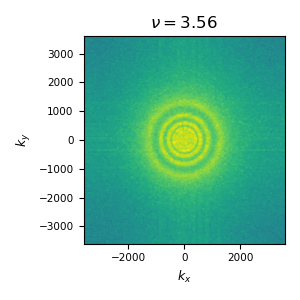
\includegraphics[width=1.0\linewidth,trim={0cm 0.4cm 0cm 0.3cm},clip=TRUE]{ring_diagram}\\
%	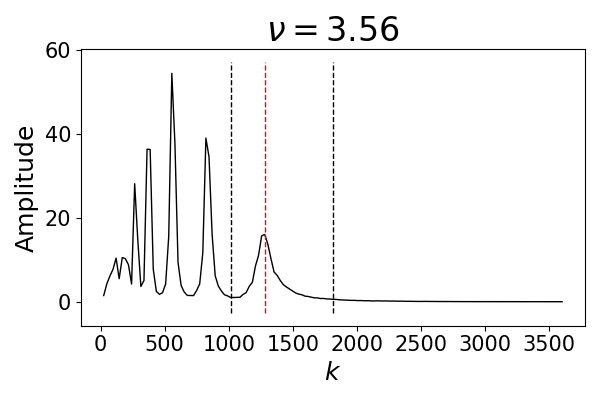
\includegraphics[width=1.0\linewidth,trim={0cm 0cm 0cm 1cm},clip=TRUE]{az_avg_spec}